\chapter{Untersuchung geeigneter Process Miner}\label{chap:approach}
Um systematisch nach einen geeigneten Algorithmus zu finden, der automatisiert Regeln aus Smart Home Prozessen extrahiert, soll eine begrenze Anzahl an Process Mining Verfahren in Testdurchläufen miteinander verglichen werden. Der Testaufbau ist derart gestaltet, dass dieser sich mit einem preisgünstigen Einplatinencomputer (Raspberry PI, etc.) in einem realen Smart Home realisieren ließe. 

\section{Auswahl Softwarelösung}
Essentiell für die Analyse ist ein Werkzeug, mit dem sich die Rohdaten über einen einheitlichen, vom verwendeten Algorithmus unabhängigen, Workflow verarbeiten lassen. Um eine geeignete Softwarelösung für die Durchführung des Prozess Mining Schritts zu bestimmen, wurden zunächst Publikationen ausgewertet, die bereits Process Mining Software unter relevanten Gesichtspunkten verglichen haben. 
Die Softwarepakete mit dem Namen ProM, Disco und Celonis sind die drei in der Literatur am häufigsten untersuchten Lösungen für den vorliegenden Anwendungsfall. Die Erkenntnisse dieser vergleichenden Studien werden in dieser Arbeit bei der Auswahl berücksichtigt und im Folgenden kurz zusammengefasst. 
Die Ergebnisse einer Veröffentlichungen der Universität Gent mit dem Titel „Process Mining in Practice: Comparative Study of Process Mining Software“ von 2014 \cite{compPM}, die durch Umfragen unter Forschern und industriellen Anwendern erforscht hat, welche Process Mining Software besonders bekannt, genutzt bzw. verbreitet ist und den Befragten am nutzerfreundlichsten erschien.

Hier zeichnen sich ProM und Disco als Führend unter den untersuchten Kandidaten ab. ProM liegt der Umfrage nach bei den Befragten in der Forschung besonders weit vorne, während Anwender in der Industrie häufiger auf kommerzielle Lösungen zurückgreift, allen voran Disco, wie der Auszug der Tabelle aus \ref{comparison} zeigt.

\begin{table}[!h]
\centering
\resizebox{0.55\textwidth}{!}{%
\begin{tabular}{l c c c }
\hline
Einsatzhäufigkeit & \textbf{Disco }& \textbf{ProM} & \textbf{Celonis} \\  
\hline\hline
häufig genutzt & 26 &  13 & 2  \\
gelegentlich genutzt & 13 &  17 & 0  \\
einmal genutzt & 6 & 12 & 0 \\
bekannt & 9  & 11 & 16  \\
unbekannt & 1 & 2 & 34  \\
\hline
\end{tabular}%
}
\caption{Auszug aus Tabelle 5 aus "Process Mining in Practice" \cite{compPM} }
\label{comparison}
\end{table}

Die Autoren der Arbeit „An Informative and Comparative Study of Process Mining Tools”, die im International Journal of Scientific and Engineering Research veröffentlicht wurde, stellen ebenfalls die oben genannten Softwarelösungen in einem Vergleich gegenüber und kommen zu dem Ergebnis, dass Celonis wie auch Disco sehr ausgereifte graphische Nutzerschnittstellen für Process Mining bieten, welche einen leichten Einstieg für unerfahrene Anwender in dem Gebiet gewährleisten, und ProM in diesem Aspekt überlegen sind. Jedoch ist ProM, aufgrund der Tatsache, dass es sich um ein Open Source Projekt handelt, das mit Abstand am umfangreichsten ausgestattete Tool hinsichtlich Konfigurationmöglichkeiten und Erweiterungen. Im Laufe seiner Entwicklung wurden zahlreiche Plugins, die verschiedenste Process Mining Algorithmen implementieren, an das Projekt angebunden und die Auswahl an Ausgabeformaten stetig erweitert, so dass das Funktionsspektrum von ProM dem von Disco oder Celonis deutlich überlegen ist, so die Autoren. Im Rahmen der Masterarbeit „Comparative Evaluation of Process Mining Tools“, die 2015 an der Universität von Tartu \cite{ComparativeEO} entstanden ist, wurden die selben drei Kandidaten anhand ihres Funktionsumfangs und ihrer Nutzerfreundlichkeit miteinander verglichen.

\begin{table}[!h]
\centering
\resizebox{\textwidth}{!}{%
\begin{tabular}{lccc}
Kriterium & \multicolumn{1}{c}{\textbf{ProM (V. 6.9)}} & \multicolumn{1}{c}{\textbf{Disco }} & \multicolumn{1}{c}{\textbf{Celonis}} \\
\hline\hline
Typ des Logs & Mxml,xes & Csv,xls, mxml, fxl & Csv,xls \\
Process Discovery & Ja & Ja & Ja \\
Lizenz & Open source & Kommerziell & Kommerziell \\
Notation der Ergebnisse & BPMN,Petri nets, EPCs, ... & Fuzzy model & Fuzzy model, Schaubilder \\
Visualisierung der Prozesse & Ja & Ja & Ja \\
Command Line Interface & Ja & Nein & Nein \\
\hline
\end{tabular}%
}
\caption{Auszug aus Tabelle 4.9 aus „Comparative Evaluation of Process Mining Tools“\cite{ComparativeEO}}
\label{comparison2}
\end{table}

Diese Arbeit kommt gleichermaßen zu dem Schluss, dass ProM ungeachtet der Gestaltung der Benutzeroberfläche den kommerziellen Kandidaten in allen Aspekten der Funktionalität überlegen ist. ProM bietet neben der Process Discovery auch Conformance Checking, sowie Social Network Mining und Trace Clustering an, und kann ermittelte Modelle als BPMN, Petri Netz und in zahlreichen weiteren Formaten darstellen, wohingegen sich Disco und Celonis auf Fuzzy Modelle beschränken. Diese Vorteile sowie die Lizenzfreiheit sind ausschlaggebend für die Entscheidung, ProM als Werkzeug in der vorliegenden Arbeit zu nutzen. 

ProM ist in der Programmiersprache Java implementiert und dessen Kernkomponente unter der GPL (GNU  Gerneral Public License) veröffentlicht. Die Dokumentation für Endanwender weist eine für gängige Szenarien ausreichende Tiefe auf, jedoch beschränkt sich die Dokumentation der Schnittstellen für Entwickler auf eine reine Aufzählung von Java-Klassen, und -Methoden, wodurch ein umfangreiches Studium des Quellcodes erforderlich ist, um eigene Erweiterungen beziehungsweise Anpassungen vorzunehmen.

Ein weiterer Vorteil von ProM ist, dass einige der integrierten Plugins eine Kommandozeilenschnittstelle bieten, mit Hilfe dieser kann die Auswertung der Eventlogs von einem Serverseitigen Skript aus gestartet und überwacht werden. Nachteilig an dieser Lösung ist allerdings, dass ProM im Gegensatz zu Disco und Celonis Eventlogs im CSV-Format (Comma Seperated Values) nicht direkt entgegen nimmt. Dadurch muss zusätzlich vorher eine Konvertierung in das XES Format stattfinden, bevor eine Process Mining Analyse durchgeführt werden kann.

\section{Wahl des Process Mining Verfahrens}

Es soll ein Process Mining Verfahren identifiziert werden, welches unter den in den Vergleich einbezogenen Minern am besten geeignet ist Modelle derart zu erzeugen, dass sie kurze, häufig auftretende Ereignis und Aktionen korrekt erkennen und abbilden. Ziel ist es, diejenigen Interaktionen mit den Smart Home Geräten des Anwenders herauszufiltern, die innerhalb eines beschränkten Zeitraums wiederholt beobachtet wurden und in einer einfachen Wenn-Dann Beziehung beschrieben werden können. 

Mining Verfahren, deren Modelle zwar korrekt, aber zu komplex sind um eine für den Anwender leicht interpretierbare Regel zu beschreiben oder solche, die auftretende Muster zu früh als Regel interpretieren, sind für diesen Anwendungsfall ungeeignet. In Anbetracht der im Eingangskapitel erläuterten Gütekriterien werden hier Modelle gefordert, die ein hohes Maß an ‚Simplicity‘ (Einfachheit) mitbringen und weniger Gewicht auf ,Fitness' legen, also kein Modell erstellen, das dazu neigt alle möglichen, selten auftretenden Prozesschritte mit einzuschließen. 

Ein weiterer Faktor, der die Auswahl an Minern einschränkt, ist die praktische Umsetzbarkeit in einer realen Anwendung. Es werden nur solche Miner berücksichtigt, für die zum Zeitpunkt dieser Arbeit ein Plugin in der ProM 6.9 Version angeboten wird und die in der Lage sind, über Kommandozeilenbefehle so aufgerufen zu werden, dass sie eine Ergebnisdatei erzeugen, ohne, dass es einer zusätzlichen Intervention seitens des Anwenders bedarf.

Für eine Vorauswahl werden Veröffentlichungen herangezogen, die sich bereits mit der Fragestellung des Process Mining von ADL auseinandergesetzt haben.

\begin{table}[!h]
\centering
\resizebox{0.9\textwidth}{!}{%
\begin{tabular}{lcccc}
 Kategorie & \textbf{Heuristic} & \textbf{Fuzzy} & \textbf{Inductive} & \textbf{Local}   \\
%Betrachtete Plugin Version & F. Mannhardt, Interactive Data Aware Heur. M. & H.M.W. Verbeek, Mine for a fuzzy Model & S.J.Leemans, Mine with Inductive Visual Miner & N.Tax, Search for Local Process Models \\
\hline\hline
Nebenläufigkeit & + & - & + & + \\
kurze Iterationen (Schleifenlänge ≤ 2) & + & + & - & + \\
Eignung für unvollständige &  &  &  &  \\
Event-Logs & + & + & + & + \\
Eignung für fehlerbehaftete &  &  &  &  \\
Event-Logs & + & + & ? & ? \\
automatisierbar & + & + &  & \\
\hline
\end{tabular}%
}
\caption{Vergleich von Process Mining Verfahren hinsichtlich ihrer Eignung für den Einsatz im Smart Home}
\label{tab:my-table}
\end{table}

Um zu untersuchen, inwieweit die Modelle der gewählten Miner sich für den im Rahmen dieser Arbeit geplanten Anwendungsfall eignen, werden sie zunächst mit künstlich erzeugten Ereignisprotokollen evaluiert. Die Testreihe setzt sich zusammen aus systematisch generierten XES Dateien, die an Ereignislogs angelehnt sind, die im Smart Home Model des ITOM Instituts entstanden sind.


\clearpage
\section{Testreihe}
\subsection{Aufbau und Durchführung}
Aufgrund der nahezu unbegrenzten Anzahl möglicher Szenarien in einem Smart Home kann nur an einem Ausschnitt an potentiell möglichen zusammengesetzten Ereignisprotokollen getestet werden. Um dennoch eine hohe Aussagekraft der Testreihe zu erhalten, sind die Ereignislogs deart gestaltet, dass sie gegenüber dem Miner inkrementell komplexer werden und so Performanzunterschiede zwischen den Algorithmen deutlich werden können. Die Abweichung zwischen gewünschtem Modell und der Ausgabe des jeweiligen Miners soll hier als Grundlage für die Bewertung dienen, um festzustellen inwieweit die untersuchten Miner geeignet sind im Smart Home Kontext zur Erzeugung von Wenn-Dann Regeln eingesetzt zu werden. 

Um eine Vergleichbarkeit mit realen Eventlos zu ermöglichen, wurden die Logs um Rauscheinträge ergänzt, welche jeweils in ihrem relativen Anteil varrieren. Zusätzlich wurde auch die Zeitspanne der Logs in Kalendertagen varriiert. Eine erfolgreiche Auswertung durch einen Miner hat stattgefunden, wenn das im Ereignisprotokoll eingebettete Muster vollständig im Modell wiedergegeben wird, parallele Abläufe korrekt dargestellt werden und keine überschüssigen (Rausch-) Einträge als Knoten im entstandenen Netz enthalten sind.

Hervorzuheben ist an dieser Stelle, dass die Miner den Inhalt einzelner Einträge nicht deuten, sie unterscheiden die Ressourcen, die den Eintrag erstellen und die zugehörigen Eigenschaften nur Anhand der Zeichenkette im Protokoll. Dementsprechend werden die Namen der IoT Ressourcen und ihrer Aktivitäten hier beispielhaft für gängige vernetzte Geräte gewählt, sie haben keine direkte Auswirkung auf das Ergebnis des Mining Verfahrens und sind beliebig austauschbar. Signifikant für die Auswertung ist zunächst nur die Häufigkeit, mit der eine Ressource einen Eintrag erstellt, und der Zeitpunkt des Eintrags im Protokoll, der zu dieser Ressource gehört.

Die Eventlogs der Testreihe werde mit Hilfe eines im Rahmen dieser Arbeit entstandenen Python Skript generiert, welches folgende Parameter entgegen nimmt: das eingebettete, zu erkennende Verhaltensmuster, die Menge an konsekutiven Kalendertagen (30 o. 90 Tage) und der Anteil an Rauscheinträgen (15 o. 50), siehe Anhang \ref{lst:generate}.

Die Testreihe setzt sich aus zwölf verschiedenen Modellen zusammen, die in künstlich erzeugte Eventlogs eingebettet werden. Diese werden inkrementell komplexer und enthalten eine jeweils unterschiedliche Menge an Knoten, die die Elemente einer Regel darstellen. Je Modell (benannt „A“ - „M“) entstehen so 4 unterschiedliche Eventlogs .Für die Durchführung der Testreihe wurden insgesamt 40 Eventlogs generiert, welche 84 individuelle Regeln enthielten; mit minimal einer, maximal vier Regeln pro Eventlog, siehe Tabellen im Anhang \ref{results}. 

\subsection{Auswertung der Messreihe}
Um die Güte der Modelle, die in der Messreihe mit den verschiedenen Minern entstanden sind zu evaluieren, werden die Ausgaben der Process Mining Plugins mit dem ursprünglich eingebetteten Modell verglichen und der Grad der Abweichung für jeden Datensatz dokumentiert.

Um die Performanz der Miner zu quantifizieren, wird  die Wiedergabe der eingebetteten Muster im Ausgabemodell über ein Punktesystem bewertet. Entspricht das Modell vollständig dem erwarteten Modell wird es mit voller Punktzahl bewertet, für Abweichungen werden Punkte abgezogen.

Als Maß für die Performanz der Miner wird die Anzahl korrekt identifizierter Regeln, die in den Eventlogs eingebettet sind, herangezogen. Für jedes der generierten Eventlogs werden die korrekt erkannten Knoten (True Positive), sowie die fälschlicherweise im Modell enthaltenen Elemente (False Postive) und diejenigen Elemente, die nicht im Modell erscheinen, aber erwartet wurden (False Negative) gezählt. 

Desweiteren ist für den Anwendungsfall von hoher Bedeutung, dass die Knoten die zu unterschiedlichen Regeln gehören auf unterschiedlichen Pfaden im Modell erscheinen. Als weitere Metrik in der Testreihe wird daher die Anzahl der korrekt erkannten Pfade im Ausgangsmodell verwendet (Parallelism). 

Entscheidend für den im Rahmen dieser Arbeit betrachteten Anwendungsfall der automatisierten Regelerkennung im Smart Home ist das der Mining Algorithmus in der Lage ist, Rauschen aus dem Modell herauszufiltern und korrekt kurze Pfade und sowie ihre Parallelität (sog. Splits) zu identifizieren. 
Die Durchführung der Testreihe hat zum Vorschein gebracht, dass es einen signifikanten Unterschied in der Fähigkeit der untersuchten Mining Algorithmen gibt, Abläufe mit vielen kurzen Pfaden zu identifizieren und im Ausgabemodell korrekt wiederzugeben. Lediglich in fünf der zehn Modelle geben beide Miner in allen vier Eventlogs das gesuchte Resultat fehlerfrei aus (konkret Reihe: A,B,D,E,F), siehe Abb.\ref{tab1} und Abb. \ref{tab2} im Anhang.

In den fünf Modellen, in denen einer der beiden Miner Plugins nicht das erwartete Modell ausgeben konnte, handelte es sich in vier Fällen (16 Eventlogs, Modell H,J,K,L,M) um das ‚Inductive Visual Miner Plugin‘, wohingegen das ‚Interactive Data-aware Heuristics Miner‘ Plugin lediglich in zwei Modellen in allen vier Eventlogs (C,G) unterlag.

Die Auswertung der Testreihe hat gezeigt, dass beide Miner gut geeignet sind bis zu zwei Regeln in einem Eventlog zu erkennen, und dass bei regelmäßigem Auftreten der Regel auch kurze Auswertungszeitspannen und ein hohes Maß an Rauscheinträgen das Ergebnismodell nicht verzerren. Dies ergibt sich aus der konsisten Ausgabequalität der Modelle über eine Messreihe hinweg. Wird die selbe Regel mehrfach in einem Eventlog eingebettet, treten nur insignifikante oder keine Unterschiede in der Ausgabe auf, unabhängig davon ob der Rauschanteil besonders hoch oder niedrig war, oder dem Miner deutlich mehr Tage zur Verfügung standen um ein Muster zu erkennen.

Im Unterschied zum Heuristic Miner Plugin gelingt es dem Inductive Miner Plugin nicht, mehr als zwei kurze Regeln korrekt in parallel verlaufende Pfaden zu unterteilen, stattdessen bestehen die resultierenden Petri Netze meist aus jeweils einem einzigen Pfad, dessen Knoten aufeinanderfolgen, und nicht wie erwartet nebeneinander verlaufen. Es gelingt dem Inductive Miner also nicht, den Split zwischen kurzen Pfaden korrekt zu setzen, sollten mehr als zwei kurze parallel verlaufende Pfade im Modell vorliegen. Da genau diese Art der Modellierung aber das gesuchte Szenario abbildet, dass ein Eventlog mehrere regelmäßige Abläufe aus zwei bis vier Eventeinträgen enthält, deuten die Ergebnisse dieser Testreihe darauf hin, dass der Heuristic Miner besser geeignet ist, kurze Regeln nach dem If This Then That Schema in einem Smart Home zu identifizieren.
\begin{figure}[!ht]
    \centering
    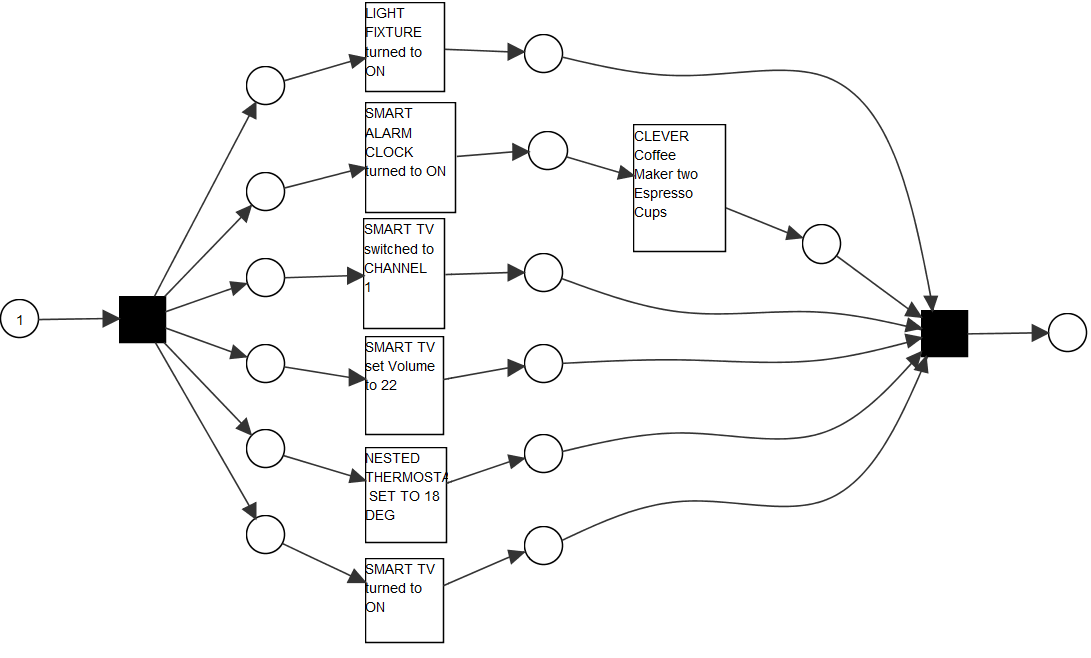
\includegraphics[width=0.7\textwidth,]{figures/Appbildungen/K_inductive_erronousPNG.PNG}
    \caption{Modellierung der Testreihe K aus dem Inductive Miner Plugin}
    \label{fig:K_inductive}
\end{figure}
Beispielhaft für diesen Fehlerfall wird das Modell 'K' betrachtet, eingebettet in die generierten Eventlogs wurden drei separate regelmäßige Wenn-Dann Abfolgen aus zwei beziehungsweise drei Elementen. Für alle vier Kombinationsmöglichkeiten zur Konfiguration des Eventlogs (30 Tage, Rauschanteil 15 oder 50 und 90 Tage mit Rauschanteil 15 oder 50) ergab der Heuristic Miner ein Modell, welches die drei erwarteten Abfolgen enthält und alle Rauscheinträge herausfiltert, wie in Abb. \ref{fig:K_heuristic} zu sehen ist.
\begin{figure}[!h]
    \centering
    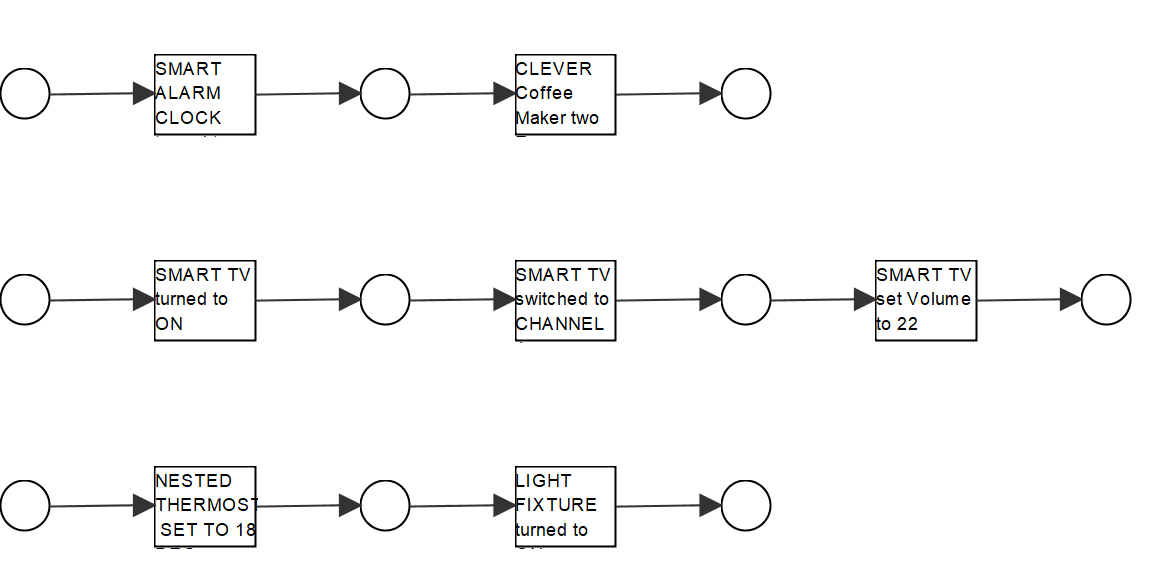
\includegraphics[width=0.7\textwidth,]{figures/Appbildungen/K_heuristic_correct.PNG}
    \caption{Modellierung der Testreihe K aus dem Heuristic Miner Plugin}
    \label{fig:K_heuristic}
\end{figure}
Auch das Inductive Miner Plugin ist in der Lage das Rauschen herauszufiltern, modelliert aber, bei Eingabe der selben Eventlog Dateien wie das Heuristic Miner Plugin, ein für den Einsatzzweck ungeeignetes Modell. 
Auf Abb. \ref{fig:K_inductive} ist zu sehen, dass nur eine Regel korrekt in der Wenn-Dann Folge abgebildet wird: auf eine 'Smart Alarm Clock' Aktivität folgt eine 'Coffee Maker' Aktivität. Die Komponenten der restlichen eingebetteten Regeln werden zwar erkannt, aber nicht in der korrekten Abfolge, sondern parallel abgebildet. Diese Form der Abweichung hat sich als charakteristisch für den Inductive Miner herausgestellt. Auch die resultierenden Modelle des Inductive Miner der Reihen H,J,L,M enthielten zwar meist die korrekten Knoten, allerdings nicht in der gewünschten Abfolge. Es entstehen vielmehr sog. Blumenmodelle, wie sie Eingangs beschrieben wurden, siehe Abschnitt \ref{quality}.

Auch der Heuristic Miner generiert nicht für jedes Eventlog das erwartete Modell, beispielsweise gelingt es ihm in der Testreihe M nicht, alle Rauscheinträge herauszufiltern, jedoch werden alle erwarteten Regeln korrekt dargestellt, siehe Abb. \ref{fig:M_heuristic}. 
Die Testreihe M enthielt nur an jedem dritten Tag Einträge zum gesuchten Muster, d.h. das Verhältnis von Rauscheinträgen zu Regeleinträgen war hier besonders hoch, was aller Wahrscheinlichkeit nach zu der fehlerhaften Modellierung geführt hat.
\begin{figure}[!ht]
    \centering
    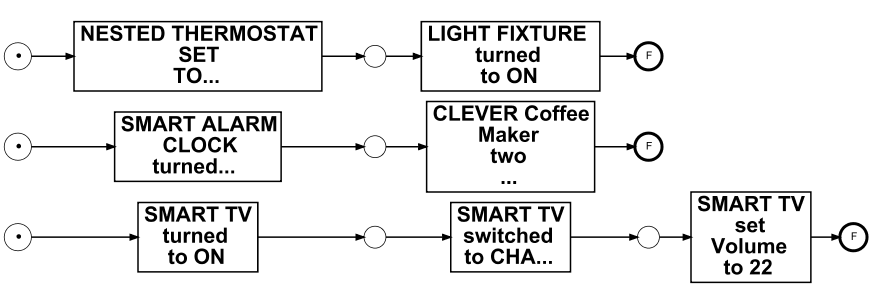
\includegraphics[width=0.7\textwidth,]{figures/Appbildungen/M_Heuristic.PNG}
    \caption{Modellierung der Testreihe M aus dem Heuristic Miner Plugin}
    \label{fig:M_heuristic}
\end{figure}
Aus der Auswertung der gesammten Testreihen geht hervor, dass aus insg. 104 Regeln, die in den 48 Eventlogs eingebettet waren, der Heuristic Miner 96 korrekt identifiziert hat, der Inductive Miner hingegen nur in 48 Fällen die gesuchten Regeln korrekt abbilden konnte.

\begin{table}[!htbp]
\centering
\resizebox{\textwidth}{!}{%
\begin{tabular}{l|ccccc}
Auswertung                & \multicolumn{1}{l}{\textbf{Testreihen}} & \multicolumn{1}{l}{\textbf{Regeln}} & \multicolumn{1}{l}{\textbf{Fehlerhafte Modelle}} & \multicolumn{1}{l}{\textbf{Identifizierte Regeln}} & \multicolumn{1}{l}{\textbf{Verfehlte Regeln}} \\ \hline
\textit{Inductive M.}  & 48                                      & 104                                 & 14                                               & 48                                                 & 56                                            \\
\textit{Heuristics M.} & 48                                      & 104                                 & 2                                                & 96                                                 & 8                                            
\end{tabular}%
}
\caption{Zusammenfassung der Auswertung der Versuchreihe}
\label{tab:results_short}
\end{table}

Desweiteren deutet die Auswertung der Testreihe darauf hin, dass der Einsatz des Heuristic Miners gegenüber dem Inductive Miner zu bevorzugen ist, wenn nach einer Modellierung gesucht wird, welche parallel und unabhängig voneinander verlaufende Prozesse in Eventlogs aufdecken soll, die jeweils aus nur wenigen, aufeinanderfolgenden Elementen bestehen.

Basierend auf den Erkenntnissen dieser Testreihe wird ein Heuristic Miner Plugin im praktischen Teil dieser Bachelorarbeit eingesetzt.




%\Rotatebox{90}{%
%\centering
%    \begin{tabular}{lp{2cm}p{2cm}p{2cm}p{2cm}p{2cm}p{2cm}}
%& Alpha Miner & Heuristic Miner & Heuristic Miner + & Fuzzy %Miner & Transition System Miner & Transition System Miner + %\\
%(garantierte) Ausführbarkeit & - & ? & ? & - & + & + \\
%Nebenläufigkeit & + & + & + & - & + & + \\
%Intervalle & - & - & + & - & + & + \\
%kurze Iterationen (Schleifenlänge ≤ 2) & - & + & + & + & + & %+ \\
%entfernte Abhängigkeiten/ nicht lokales Verhalten & - & + & + %& + & + & + \\
%nicht wahrnehmbare Aktivitäten & - & + & + & - & + & + \\
%Eignung für unvollständige Event Logs & - & + & + & + & + & + %\\
%Eignung für fehlerbehaftete Event Logs & - & + & + & + & - & %- \\
%Frequenz von Traces wird berücksichtigt & - & + & + & ? & - & %+ \\
%parametrisierbar & - & + & + & + & + & + \\
%automatisierbar & + & - & - & - & - & + \\
%tolerant gegenüber unstrukturierten Prozessen & - & ? & ? & + %& - & - \\
%ein Mining-Schritt & + & + & + & + & - & - \\
%zwei Mining-Schritte & - & - & - & - & + & + \\
%Ausgabeformat & & & & & & \\
%Petri-Netz & + & - & - & - & + & + \\
%heuristisches Netz & - & + & + & - & - & - \\
%Fuzzy-Modell & - & - & - & + & - & - \\
%Transitionssystem & - & - & - & - & + & + \\
%\end{tabular} 
%}

%\begin{table}[h!]
%\centering
%\begin{tabular}{ccccccc}
%& Alpha Miner & Heuristic Miner & Heuristic Miner + & Fuzzy Miner & Transition System Miner %& Transition System Miner + \\
%(garantierte) Ausführbarkeit & - & ? & ? & - & + & + \\
%Nebenläufigkeit & + & + & + & - & + & + \\
%Intervalle & - & - & + & - & + & + \\
%kurze Iterationen (Schleifenlänge ≤ 2) & - & + & + & + & + & + \\
%entfernte Abhängigkeiten/ nicht lokales Verhalten & - & + & + & + & + & + \\
%nicht wahrnehmbare Aktivitäten & - & + & + & - & + & + \\
%Eignung für unvollständige Event Logs & - & + & + & + & + & + \\
%Eignung für fehlerbehaftete Event Logs & - & + & + & + & - & - \\
%Frequenz von Traces wird berücksichtigt & - & + & + & ? & - & + \\
%parametrisierbar & - & + & + & + & + & + \\
%automatisierbar & + & - & - & - & - & + \\
%tolerant gegenüber unstrukturierten Prozessen & - & ? & ? & + & - & - \\
%ein Mining-Schritt & + & + & + & + & - & - \\
%zwei Mining-Schritte & - & - & - & - & + & + \\
%Ausgabeformat & & & & & & \\
%Petri-Netz & + & - & - & - & + & + \\
%heuristisches Netz & - & + & + & - & - & - \\
%Fuzzy-Modell & - & - & - & + & - & - \\
%Transitionssystem & - & - & - & - & + & + \\
%\end{tabular} 
%\caption{Eigenschaften der wichtigsten Mining Algorithmen}
%\label{table:1}
%\end{table}